\subsection{Architektur und Aufbau}
Die App „Locals“ ist eine mobile Anwendung, die Nutzer:innen dabei unterstützt,
lokale Events zu entdecken, zu erstellen und zu verwalten. Sie richtet sich an
ein junges, urbanes Publikum und zielt darauf ab, soziale Interaktionen rund um
Veranstaltungen zu fördern.

% \begin{figure}[htbp]
%     \centering
%     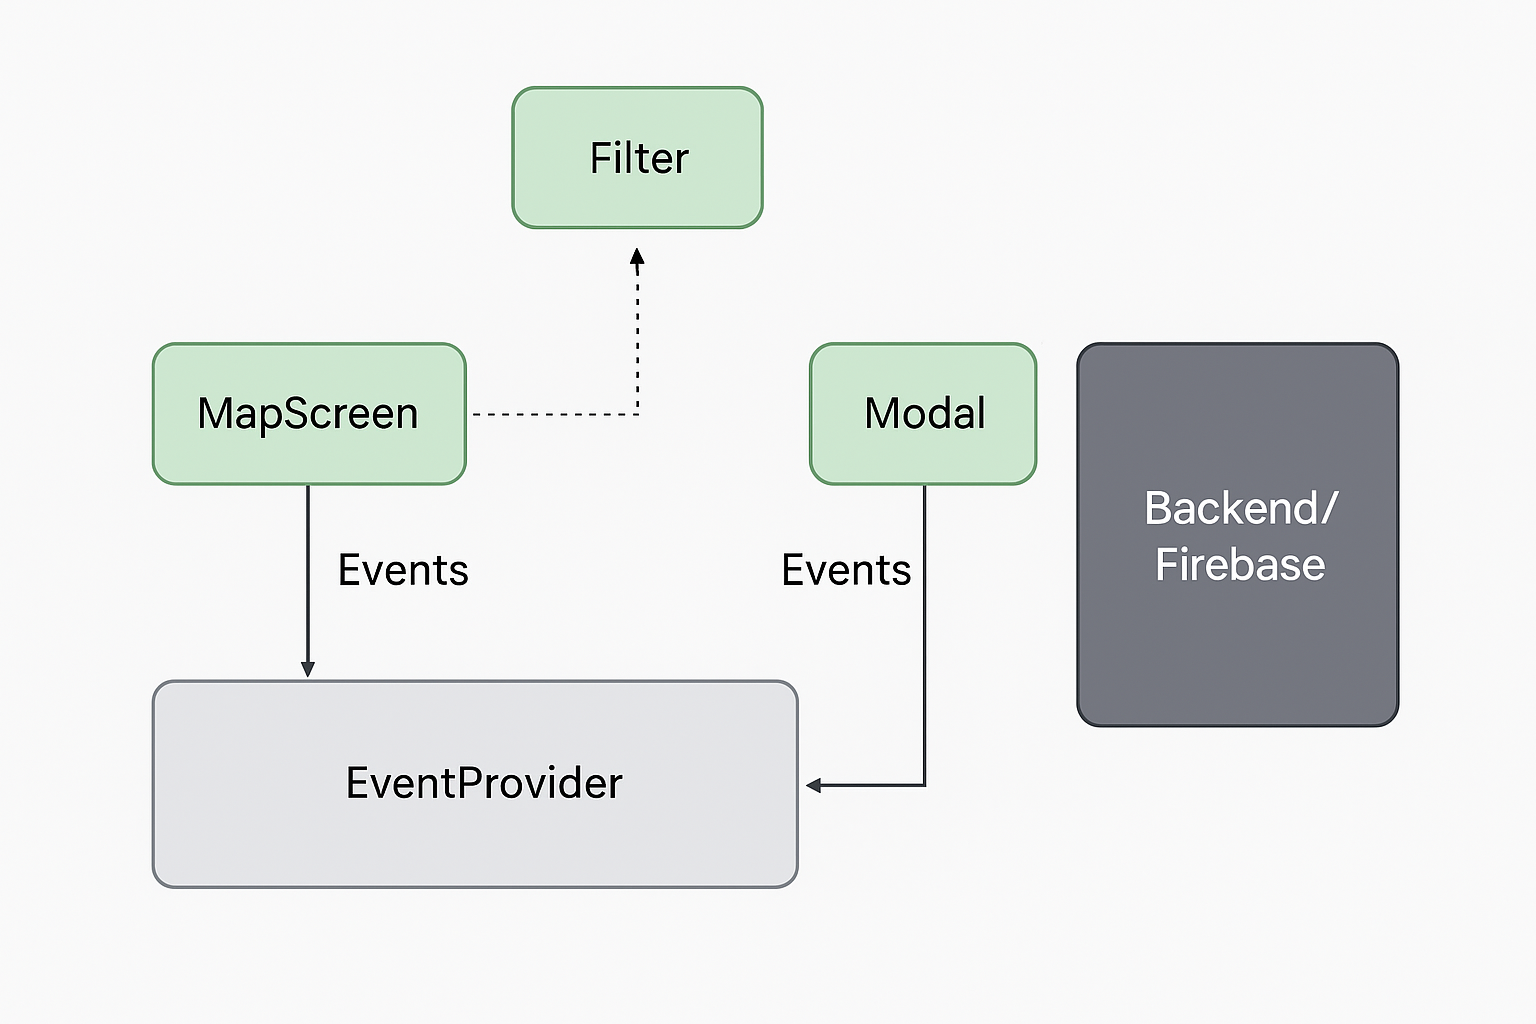
\includegraphics[width=0.95\textwidth]{images/architekturdiagramm_locals.png}
%     \caption{Architektur der App „Locals“: Darstellung der Hauptkomponenten (MapScreen, Filter, Modal, EventProvider, Backend/Firebase) und deren Datenflüsse.
%     \label{fig:architektur-locals}
% \end{figure}

\subsubsection{Technologischer Stack und Architektur}

\begin{itemize}
    \item \textbf{Frontend:} Entwicklung mit React Native, TypeScript und Expo zur plattformübergreifenden Bereitstellung für iOS und Android.
    \item \textbf{Backend:} Nutzung von Firebase für Authentifizierung, Datenhaltung und Synchronisation.
    \item \textbf{Navigation:} Einsatz von \texttt{@react-navigation/native} und \texttt{expo-router} für ein modernes, tab-basiertes Navigationskonzept.
    \item \textbf{State-Management:} Eigene Context-Provider (\texttt{AuthProvider}, \texttt{EventsProvider}) für Authentifizierungs- und Eventdaten.
    \item \textbf{UI-Komponenten:} Verwendung von \texttt{@expo/vector-icons} und \texttt{lucide-react-native} zur Gestaltung eines ansprechenden User Interface.
    \item \textbf{Maps \& Location:} Die Integration von \texttt{react-native-maps} und \texttt{expo-location} ermöglicht eine interaktive Kartenansicht, die sowohl den Nutzerstandort als auch Events auf einer Karte anzeigt.
\end{itemize}

Die App ist modular aufgebaut und umfasst drei zentrale Bereiche:
\begin{itemize}
    \item \textbf{Explore-Screen:} Event-Feed nach Interessen und Standort
    \item \textbf{Map-Screen:} Interaktive Kartenansicht mit Event-Markern und Filterfunktion
    \item \textbf{Profil-Screen:} Persönliche Eventübersicht und Verwaltung
\end{itemize}

Während der Explore- und Profil-Screen bereits Grundfunktionen aufweisen, wird
der Map-Screen im Rahmen dieser Arbeit als prototypisches
Demonstrationsbeispiel gezielt entwickelt und evaluiert. Die praktische
Realisierung dieses Features erfolgt unter Einsatz generativer KI-Tools und
steht im Mittelpunkt der anschließenden Kapitel.

\subsubsection{Struktur der Haupteinstiegskomponente (RootLayout)}
Die zentrale Einstiegskomponente der App ist das \texttt{RootLayout}. Sie
übernimmt das Laden benutzerdefinierter Fonts, die Einbindung von
Authentifizierungs- und Events-Kontexten sowie die nahtlose Nutzerführung nach
dem Login. Die Navigation wird dabei strikt vom Authentifizierungsstatus
gesteuert, sodass nicht eingeloggte Nutzer:innen automatisch zur Login-Ansicht
weitergeleitet werden. Dies wird mit Hilfe der Hooks \texttt{useAuth},
\texttt{useSegments} und \texttt{useRouter} umgesetzt.

\subsection{Bestehende Funktionalitäten}
Zu den bereits implementierten Basisfunktionen von Locals gehören:
\begin{itemize}
    \item \textbf{Benutzerauthentifizierung:} Sichere Registrierung und Anmeldung über Firebase Authentication.
    \item \textbf{Profilverwaltung:} Verwaltung persönlicher Daten sowie Übersicht über besuchte und selbst erstellte Events.
    \item \textbf{Eventverwaltung:} Anlegen, Bearbeiten und Löschen von Events.
    \item \textbf{Tab-Navigation:} Ermöglicht den nahtlosen Wechsel zwischen den drei Hauptbereichen „Explore“, „Map“ und „Profil“.
    \item \textbf{Responsives Design:} Durch Nutzung von \texttt{react-native-safe-area-context} und Expo UI-Komponenten wird eine konsistente Darstellung auf unterschiedlichen Geräten gewährleistet.
\end{itemize}

Der Map-Screen ist als zentrales, innovatives Feature der App konzipiert. Die
Implementierung und Weiterentwicklung dieses Moduls wird im weiteren Verlauf
dieser Arbeit als praktisches Beispiel für den Einsatz generativer KI in der
Softwareentwicklung demonstriert und analysiert.
